% 2021-11-20
\begin{exercise}
      {ID-16b0d9ae80b9c0af9854636110bb8c20fd4be148}
      {Eine passende Situation}
  \ifproblem\problem\par
    % <PROBLEM>
    Gegeben ist folgendes Prozessdiagramm:
    \begin{center}
      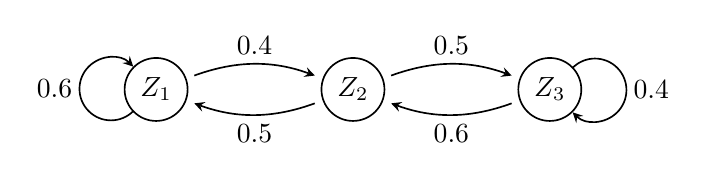
\begin{tikzpicture}[line width=0.6pt]
        \node[shape=circle,
              minimum size=8mm,
              inner sep=0pt,
              draw=black] (Z1) at (0, 0) {$Z_1$};
        \node[shape=circle,
              minimum size=8mm,
              inner sep=0pt,
              draw=black] (Z2) at (2.5, 0) {$Z_2$};
        \node[shape=circle,
              minimum size=8mm,
              inner sep=0pt,
              draw=black] (Z3) at (5, 0) {$Z_3$};
        %<OCTAVE>
        \draw[<-, >=stealth] (Z1.135.000)
              arc[start angle=45.000,
                  end angle=315.000,
                  radius=4.000mm]
              node[pos=0.5,
                   shift={(180.000:9pt)}]
                   {\num{0.6}};
        %</OCTAVE>
        %myselfconnect("Z1", 180);
        %<OCTAVE>
        \draw[<-, >=stealth] (Z3.315.000)
              arc[start angle=225.000,
                  end angle=495.000,
                  radius=4.000mm]
              node[pos=0.5,
                   shift={(0.000:9pt)}]
                   {\num{0.4}};
        %</OCTAVE>
        %myselfconnect("Z3", 0);
        \begin{scope}[->, >=stealth, shorten <=3pt, shorten >=3pt]
          \draw (Z1.20) to[out=20, in=160]
                        node[above] {\num{0.4}}
                (Z2.160);
          \draw (Z2.200) to[out=200, in=340]
                         node[below] {\num{0.5}}
                (Z1.340);
          \draw (Z2.20) to[out=20, in=160]
                        node[above] {\num{0.5}}
                (Z3.160);
          \draw (Z3.200) to[out=200, in=340]
                         node[below] {\num{0.6}}
                (Z2.340);
        \end{scope}
      \end{tikzpicture}
    \end{center}
    \begin{enumerate}[a)]
      \item Stellen Sie die Übergansmatrix $U$ zu
            diesem Prozessdiagramm auf.
            Überprüfen Sie, ob $U$ eine stochastische
            Matrix ist.
      \item $Z_1$ wird als Anfangszustand gewählt.
            Bestimmen Sie damit die Zustandsverteilung
            nach vier Schritten.
      \item Beschreiben Sie eine Situation, die zu dem
            Diagramm passt.
      \item Verändern Sie die Übergangswahrscheinlichkeiten
            so, dass $Z_1$ und $Z_3$ absorbierende
            Zustände sind.
    \end{enumerate}
    % </PROBLEM>
  \fi
  %\ifoutline\outline\par
    % <OUTLINE>
    % </OUTLINE>
  %\fi
  %\ifoutcome\outcome\par
    % <OUTCOME>
    % </OUTCOME>
  %\fi
\end{exercise}
